% Created by tikzDevice version 0.12.3 on 2019-08-15 12:03:26
% !TEX encoding = UTF-8 Unicode
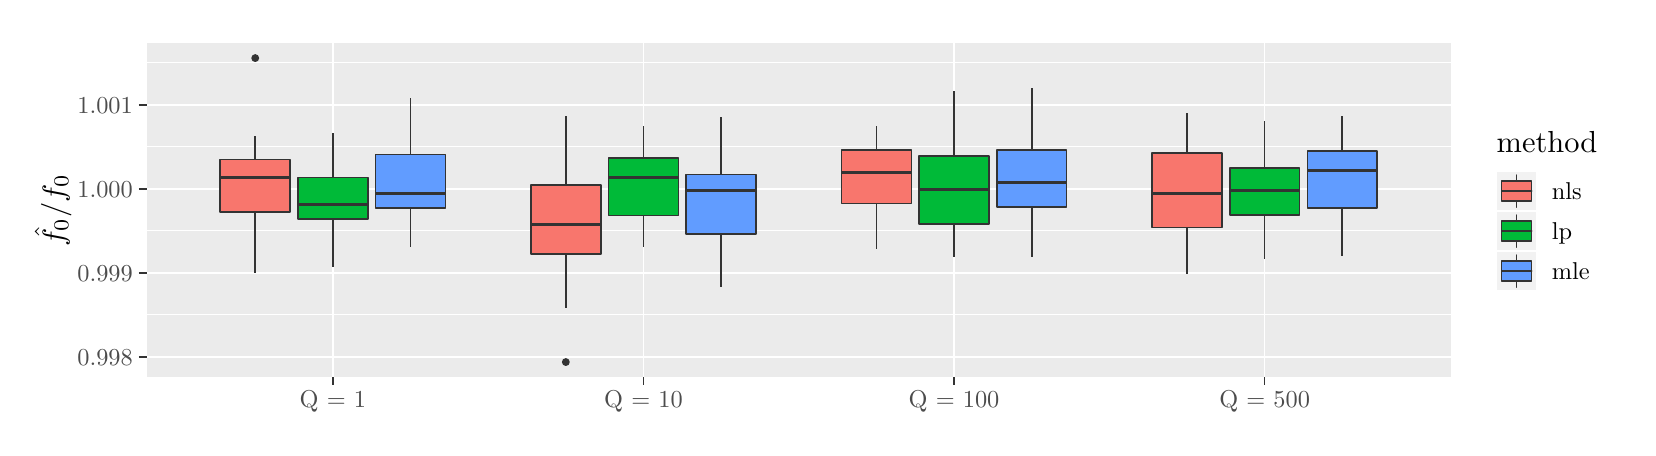
\begin{tikzpicture}[x=1pt,y=1pt]
\definecolor{fillColor}{RGB}{255,255,255}
\path[use as bounding box,fill=fillColor,fill opacity=0.00] (0,0) rectangle (578.16,144.54);
\begin{scope}
\path[clip] (  0.00,  0.00) rectangle (578.16,144.54);
\definecolor{drawColor}{RGB}{255,255,255}
\definecolor{fillColor}{RGB}{255,255,255}

\path[draw=drawColor,line width= 0.6pt,line join=round,line cap=round,fill=fillColor] (  0.00,  0.00) rectangle (578.16,144.54);
\end{scope}
\begin{scope}
\path[clip] ( 42.95, 18.22) rectangle (514.31,139.04);
\definecolor{fillColor}{gray}{0.92}

\path[fill=fillColor] ( 42.95, 18.22) rectangle (514.31,139.04);
\definecolor{drawColor}{RGB}{255,255,255}

\path[draw=drawColor,line width= 0.3pt,line join=round] ( 42.95, 40.78) --
	(514.31, 40.78);

\path[draw=drawColor,line width= 0.3pt,line join=round] ( 42.95, 71.14) --
	(514.31, 71.14);

\path[draw=drawColor,line width= 0.3pt,line join=round] ( 42.95,101.51) --
	(514.31,101.51);

\path[draw=drawColor,line width= 0.3pt,line join=round] ( 42.95,131.87) --
	(514.31,131.87);

\path[draw=drawColor,line width= 0.6pt,line join=round] ( 42.95, 25.59) --
	(514.31, 25.59);

\path[draw=drawColor,line width= 0.6pt,line join=round] ( 42.95, 55.96) --
	(514.31, 55.96);

\path[draw=drawColor,line width= 0.6pt,line join=round] ( 42.95, 86.32) --
	(514.31, 86.32);

\path[draw=drawColor,line width= 0.6pt,line join=round] ( 42.95,116.69) --
	(514.31,116.69);

\path[draw=drawColor,line width= 0.6pt,line join=round] (110.29, 18.22) --
	(110.29,139.04);

\path[draw=drawColor,line width= 0.6pt,line join=round] (222.52, 18.22) --
	(222.52,139.04);

\path[draw=drawColor,line width= 0.6pt,line join=round] (334.74, 18.22) --
	(334.74,139.04);

\path[draw=drawColor,line width= 0.6pt,line join=round] (446.97, 18.22) --
	(446.97,139.04);
\definecolor{drawColor}{gray}{0.20}
\definecolor{fillColor}{gray}{0.20}

\path[draw=drawColor,line width= 0.4pt,line join=round,line cap=round,fill=fillColor] ( 82.23,133.55) circle (  1.21);

\path[draw=drawColor,line width= 0.6pt,line join=round] ( 82.23, 96.87) -- ( 82.23,105.52);

\path[draw=drawColor,line width= 0.6pt,line join=round] ( 82.23, 77.88) -- ( 82.23, 55.78);
\definecolor{fillColor}{RGB}{248,118,109}

\path[draw=drawColor,line width= 0.6pt,line join=round,line cap=round,fill=fillColor] ( 69.61, 96.87) --
	( 69.61, 77.88) --
	( 94.86, 77.88) --
	( 94.86, 96.87) --
	( 69.61, 96.87) --
	cycle;

\path[draw=drawColor,line width= 1.1pt,line join=round] ( 69.61, 90.46) -- ( 94.86, 90.46);

\path[draw=drawColor,line width= 0.6pt,line join=round] (110.29, 90.36) -- (110.29,106.42);

\path[draw=drawColor,line width= 0.6pt,line join=round] (110.29, 75.31) -- (110.29, 57.89);
\definecolor{fillColor}{RGB}{0,186,56}

\path[draw=drawColor,line width= 0.6pt,line join=round,line cap=round,fill=fillColor] ( 97.66, 90.36) --
	( 97.66, 75.31) --
	(122.92, 75.31) --
	(122.92, 90.36) --
	( 97.66, 90.36) --
	cycle;

\path[draw=drawColor,line width= 1.1pt,line join=round] ( 97.66, 80.56) -- (122.92, 80.56);

\path[draw=drawColor,line width= 0.6pt,line join=round] (138.35, 98.69) -- (138.35,119.05);

\path[draw=drawColor,line width= 0.6pt,line join=round] (138.35, 79.41) -- (138.35, 65.12);
\definecolor{fillColor}{RGB}{97,156,255}

\path[draw=drawColor,line width= 0.6pt,line join=round,line cap=round,fill=fillColor] (125.72, 98.69) --
	(125.72, 79.41) --
	(150.97, 79.41) --
	(150.97, 98.69) --
	(125.72, 98.69) --
	cycle;

\path[draw=drawColor,line width= 1.1pt,line join=round] (125.72, 84.74) -- (150.97, 84.74);
\definecolor{fillColor}{gray}{0.20}

\path[draw=drawColor,line width= 0.4pt,line join=round,line cap=round,fill=fillColor] (194.46, 23.71) circle (  1.21);

\path[draw=drawColor,line width= 0.6pt,line join=round] (194.46, 87.68) -- (194.46,112.54);

\path[draw=drawColor,line width= 0.6pt,line join=round] (194.46, 62.87) -- (194.46, 43.29);
\definecolor{fillColor}{RGB}{248,118,109}

\path[draw=drawColor,line width= 0.6pt,line join=round,line cap=round,fill=fillColor] (181.83, 87.68) --
	(181.83, 62.87) --
	(207.09, 62.87) --
	(207.09, 87.68) --
	(181.83, 87.68) --
	cycle;

\path[draw=drawColor,line width= 1.1pt,line join=round] (181.83, 73.47) -- (207.09, 73.47);

\path[draw=drawColor,line width= 0.6pt,line join=round] (222.52, 97.53) -- (222.52,109.05);

\path[draw=drawColor,line width= 0.6pt,line join=round] (222.52, 76.72) -- (222.52, 65.23);
\definecolor{fillColor}{RGB}{0,186,56}

\path[draw=drawColor,line width= 0.6pt,line join=round,line cap=round,fill=fillColor] (209.89, 97.53) --
	(209.89, 76.72) --
	(235.14, 76.72) --
	(235.14, 97.53) --
	(209.89, 97.53) --
	cycle;

\path[draw=drawColor,line width= 1.1pt,line join=round] (209.89, 90.39) -- (235.14, 90.39);

\path[draw=drawColor,line width= 0.6pt,line join=round] (250.57, 91.50) -- (250.57,112.41);

\path[draw=drawColor,line width= 0.6pt,line join=round] (250.57, 70.00) -- (250.57, 50.77);
\definecolor{fillColor}{RGB}{97,156,255}

\path[draw=drawColor,line width= 0.6pt,line join=round,line cap=round,fill=fillColor] (237.95, 91.50) --
	(237.95, 70.00) --
	(263.20, 70.00) --
	(263.20, 91.50) --
	(237.95, 91.50) --
	cycle;

\path[draw=drawColor,line width= 1.1pt,line join=round] (237.95, 85.77) -- (263.20, 85.77);

\path[draw=drawColor,line width= 0.6pt,line join=round] (306.69,100.28) -- (306.69,109.05);

\path[draw=drawColor,line width= 0.6pt,line join=round] (306.69, 81.02) -- (306.69, 64.74);
\definecolor{fillColor}{RGB}{248,118,109}

\path[draw=drawColor,line width= 0.6pt,line join=round,line cap=round,fill=fillColor] (294.06,100.28) --
	(294.06, 81.02) --
	(319.31, 81.02) --
	(319.31,100.28) --
	(294.06,100.28) --
	cycle;

\path[draw=drawColor,line width= 1.1pt,line join=round] (294.06, 92.33) -- (319.31, 92.33);

\path[draw=drawColor,line width= 0.6pt,line join=round] (334.74, 98.24) -- (334.74,121.55);

\path[draw=drawColor,line width= 0.6pt,line join=round] (334.74, 73.68) -- (334.74, 61.83);
\definecolor{fillColor}{RGB}{0,186,56}

\path[draw=drawColor,line width= 0.6pt,line join=round,line cap=round,fill=fillColor] (322.12, 98.24) --
	(322.12, 73.68) --
	(347.37, 73.68) --
	(347.37, 98.24) --
	(322.12, 98.24) --
	cycle;

\path[draw=drawColor,line width= 1.1pt,line join=round] (322.12, 86.15) -- (347.37, 86.15);

\path[draw=drawColor,line width= 0.6pt,line join=round] (362.80,100.38) -- (362.80,122.69);

\path[draw=drawColor,line width= 0.6pt,line join=round] (362.80, 79.63) -- (362.80, 61.65);
\definecolor{fillColor}{RGB}{97,156,255}

\path[draw=drawColor,line width= 0.6pt,line join=round,line cap=round,fill=fillColor] (350.18,100.38) --
	(350.18, 79.63) --
	(375.43, 79.63) --
	(375.43,100.38) --
	(350.18,100.38) --
	cycle;

\path[draw=drawColor,line width= 1.1pt,line join=round] (350.18, 88.61) -- (375.43, 88.61);

\path[draw=drawColor,line width= 0.6pt,line join=round] (418.91, 99.19) -- (418.91,113.72);

\path[draw=drawColor,line width= 0.6pt,line join=round] (418.91, 72.32) -- (418.91, 55.36);
\definecolor{fillColor}{RGB}{248,118,109}

\path[draw=drawColor,line width= 0.6pt,line join=round,line cap=round,fill=fillColor] (406.29, 99.19) --
	(406.29, 72.32) --
	(431.54, 72.32) --
	(431.54, 99.19) --
	(406.29, 99.19) --
	cycle;

\path[draw=drawColor,line width= 1.1pt,line join=round] (406.29, 84.53) -- (431.54, 84.53);

\path[draw=drawColor,line width= 0.6pt,line join=round] (446.97, 93.87) -- (446.97,110.97);

\path[draw=drawColor,line width= 0.6pt,line join=round] (446.97, 76.93) -- (446.97, 60.84);
\definecolor{fillColor}{RGB}{0,186,56}

\path[draw=drawColor,line width= 0.6pt,line join=round,line cap=round,fill=fillColor] (434.35, 93.87) --
	(434.35, 76.93) --
	(459.60, 76.93) --
	(459.60, 93.87) --
	(434.35, 93.87) --
	cycle;

\path[draw=drawColor,line width= 1.1pt,line join=round] (434.35, 85.66) -- (459.60, 85.66);

\path[draw=drawColor,line width= 0.6pt,line join=round] (475.03, 99.88) -- (475.03,112.52);

\path[draw=drawColor,line width= 0.6pt,line join=round] (475.03, 79.28) -- (475.03, 62.19);
\definecolor{fillColor}{RGB}{97,156,255}

\path[draw=drawColor,line width= 0.6pt,line join=round,line cap=round,fill=fillColor] (462.40, 99.88) --
	(462.40, 79.28) --
	(487.65, 79.28) --
	(487.65, 99.88) --
	(462.40, 99.88) --
	cycle;

\path[draw=drawColor,line width= 1.1pt,line join=round] (462.40, 93.09) -- (487.65, 93.09);
\end{scope}
\begin{scope}
\path[clip] (  0.00,  0.00) rectangle (578.16,144.54);
\definecolor{drawColor}{gray}{0.30}

\node[text=drawColor,anchor=base east,inner sep=0pt, outer sep=0pt, scale=  0.88] at ( 38.00, 22.56) {0.998};

\node[text=drawColor,anchor=base east,inner sep=0pt, outer sep=0pt, scale=  0.88] at ( 38.00, 52.93) {0.999};

\node[text=drawColor,anchor=base east,inner sep=0pt, outer sep=0pt, scale=  0.88] at ( 38.00, 83.29) {1.000};

\node[text=drawColor,anchor=base east,inner sep=0pt, outer sep=0pt, scale=  0.88] at ( 38.00,113.66) {1.001};
\end{scope}
\begin{scope}
\path[clip] (  0.00,  0.00) rectangle (578.16,144.54);
\definecolor{drawColor}{gray}{0.20}

\path[draw=drawColor,line width= 0.6pt,line join=round] ( 40.20, 25.59) --
	( 42.95, 25.59);

\path[draw=drawColor,line width= 0.6pt,line join=round] ( 40.20, 55.96) --
	( 42.95, 55.96);

\path[draw=drawColor,line width= 0.6pt,line join=round] ( 40.20, 86.32) --
	( 42.95, 86.32);

\path[draw=drawColor,line width= 0.6pt,line join=round] ( 40.20,116.69) --
	( 42.95,116.69);
\end{scope}
\begin{scope}
\path[clip] (  0.00,  0.00) rectangle (578.16,144.54);
\definecolor{drawColor}{gray}{0.20}

\path[draw=drawColor,line width= 0.6pt,line join=round] (110.29, 15.47) --
	(110.29, 18.22);

\path[draw=drawColor,line width= 0.6pt,line join=round] (222.52, 15.47) --
	(222.52, 18.22);

\path[draw=drawColor,line width= 0.6pt,line join=round] (334.74, 15.47) --
	(334.74, 18.22);

\path[draw=drawColor,line width= 0.6pt,line join=round] (446.97, 15.47) --
	(446.97, 18.22);
\end{scope}
\begin{scope}
\path[clip] (  0.00,  0.00) rectangle (578.16,144.54);
\definecolor{drawColor}{gray}{0.30}

\node[text=drawColor,anchor=base,inner sep=0pt, outer sep=0pt, scale=  0.88] at (110.29,  7.21) {Q = 1};

\node[text=drawColor,anchor=base,inner sep=0pt, outer sep=0pt, scale=  0.88] at (222.52,  7.21) {Q = 10};

\node[text=drawColor,anchor=base,inner sep=0pt, outer sep=0pt, scale=  0.88] at (334.74,  7.21) {Q = 100};

\node[text=drawColor,anchor=base,inner sep=0pt, outer sep=0pt, scale=  0.88] at (446.97,  7.21) {Q = 500};
\end{scope}
\begin{scope}
\path[clip] (  0.00,  0.00) rectangle (578.16,144.54);
\definecolor{drawColor}{RGB}{0,0,0}

\node[text=drawColor,rotate= 90.00,anchor=base,inner sep=0pt, outer sep=0pt, scale=  1.10] at ( 13.08, 78.63) {$\hat{f_0}/f_0$};
\end{scope}
\begin{scope}
\path[clip] (  0.00,  0.00) rectangle (578.16,144.54);
\definecolor{fillColor}{RGB}{255,255,255}

\path[fill=fillColor] (525.31, 43.84) rectangle (572.66,113.42);
\end{scope}
\begin{scope}
\path[clip] (  0.00,  0.00) rectangle (578.16,144.54);
\definecolor{drawColor}{RGB}{0,0,0}

\node[text=drawColor,anchor=base west,inner sep=0pt, outer sep=0pt, scale=  1.10] at (530.81, 99.27) {method};
\end{scope}
\begin{scope}
\path[clip] (  0.00,  0.00) rectangle (578.16,144.54);
\definecolor{drawColor}{RGB}{255,255,255}
\definecolor{fillColor}{gray}{0.95}

\path[draw=drawColor,line width= 0.6pt,line join=round,line cap=round,fill=fillColor] (530.81, 78.25) rectangle (545.26, 92.70);
\end{scope}
\begin{scope}
\path[clip] (  0.00,  0.00) rectangle (578.16,144.54);
\definecolor{drawColor}{gray}{0.20}

\path[draw=drawColor,line width= 0.6pt,line join=round,line cap=round] (538.03, 79.70) --
	(538.03, 81.86);

\path[draw=drawColor,line width= 0.6pt,line join=round,line cap=round] (538.03, 89.09) --
	(538.03, 91.26);
\definecolor{fillColor}{RGB}{248,118,109}

\path[draw=drawColor,line width= 0.6pt,line join=round,line cap=round,fill=fillColor] (532.61, 81.86) rectangle (543.45, 89.09);

\path[draw=drawColor,line width= 0.6pt,line join=round,line cap=round] (532.61, 85.48) --
	(543.45, 85.48);
\end{scope}
\begin{scope}
\path[clip] (  0.00,  0.00) rectangle (578.16,144.54);
\definecolor{drawColor}{RGB}{255,255,255}
\definecolor{fillColor}{gray}{0.95}

\path[draw=drawColor,line width= 0.6pt,line join=round,line cap=round,fill=fillColor] (530.81, 63.80) rectangle (545.26, 78.25);
\end{scope}
\begin{scope}
\path[clip] (  0.00,  0.00) rectangle (578.16,144.54);
\definecolor{drawColor}{gray}{0.20}

\path[draw=drawColor,line width= 0.6pt,line join=round,line cap=round] (538.03, 65.24) --
	(538.03, 67.41);

\path[draw=drawColor,line width= 0.6pt,line join=round,line cap=round] (538.03, 74.64) --
	(538.03, 76.81);
\definecolor{fillColor}{RGB}{0,186,56}

\path[draw=drawColor,line width= 0.6pt,line join=round,line cap=round,fill=fillColor] (532.61, 67.41) rectangle (543.45, 74.64);

\path[draw=drawColor,line width= 0.6pt,line join=round,line cap=round] (532.61, 71.02) --
	(543.45, 71.02);
\end{scope}
\begin{scope}
\path[clip] (  0.00,  0.00) rectangle (578.16,144.54);
\definecolor{drawColor}{RGB}{255,255,255}
\definecolor{fillColor}{gray}{0.95}

\path[draw=drawColor,line width= 0.6pt,line join=round,line cap=round,fill=fillColor] (530.81, 49.34) rectangle (545.26, 63.80);
\end{scope}
\begin{scope}
\path[clip] (  0.00,  0.00) rectangle (578.16,144.54);
\definecolor{drawColor}{gray}{0.20}

\path[draw=drawColor,line width= 0.6pt,line join=round,line cap=round] (538.03, 50.79) --
	(538.03, 52.96);

\path[draw=drawColor,line width= 0.6pt,line join=round,line cap=round] (538.03, 60.18) --
	(538.03, 62.35);
\definecolor{fillColor}{RGB}{97,156,255}

\path[draw=drawColor,line width= 0.6pt,line join=round,line cap=round,fill=fillColor] (532.61, 52.96) rectangle (543.45, 60.18);

\path[draw=drawColor,line width= 0.6pt,line join=round,line cap=round] (532.61, 56.57) --
	(543.45, 56.57);
\end{scope}
\begin{scope}
\path[clip] (  0.00,  0.00) rectangle (578.16,144.54);
\definecolor{drawColor}{RGB}{0,0,0}

\node[text=drawColor,anchor=base west,inner sep=0pt, outer sep=0pt, scale=  0.88] at (550.76, 82.45) {nls};
\end{scope}
\begin{scope}
\path[clip] (  0.00,  0.00) rectangle (578.16,144.54);
\definecolor{drawColor}{RGB}{0,0,0}

\node[text=drawColor,anchor=base west,inner sep=0pt, outer sep=0pt, scale=  0.88] at (550.76, 67.99) {lp};
\end{scope}
\begin{scope}
\path[clip] (  0.00,  0.00) rectangle (578.16,144.54);
\definecolor{drawColor}{RGB}{0,0,0}

\node[text=drawColor,anchor=base west,inner sep=0pt, outer sep=0pt, scale=  0.88] at (550.76, 53.54) {mle};
\end{scope}
\end{tikzpicture}
